\subsection{Use Case 3: Scan Skin}

    \subsubsection{General Description}
    
        \begin{tabular}{|p{.2\linewidth}|p{.65\linewidth}|}
        \hline 
        ID: & Scan Skin \\ \hline
        Goal: & To let the user submit a picture so an diagnosis can be made \\ \hline
        Precondition: & The user selected the Scan Skin feature from the burger menu or it got recommend in the chat based on an previous diagnosis  \\ \hline
        Postcondition: & The user can now get an diagnosis based on their picture \\ \hline
        Involved Users: & User:  Someone who uses our app \\ \hline
        \end{tabular}
    
    \subsubsection{UI to call the use case}
        
        There are two ways a user can open our skin scan feature:
        
        \begin{enumerate}
        \item The user opens our app with the intent to check their skin and starts the process of getting a diagnosis by clicking on the menu icon and selecting the camera icon to start taking a picture and submitting it.
            
            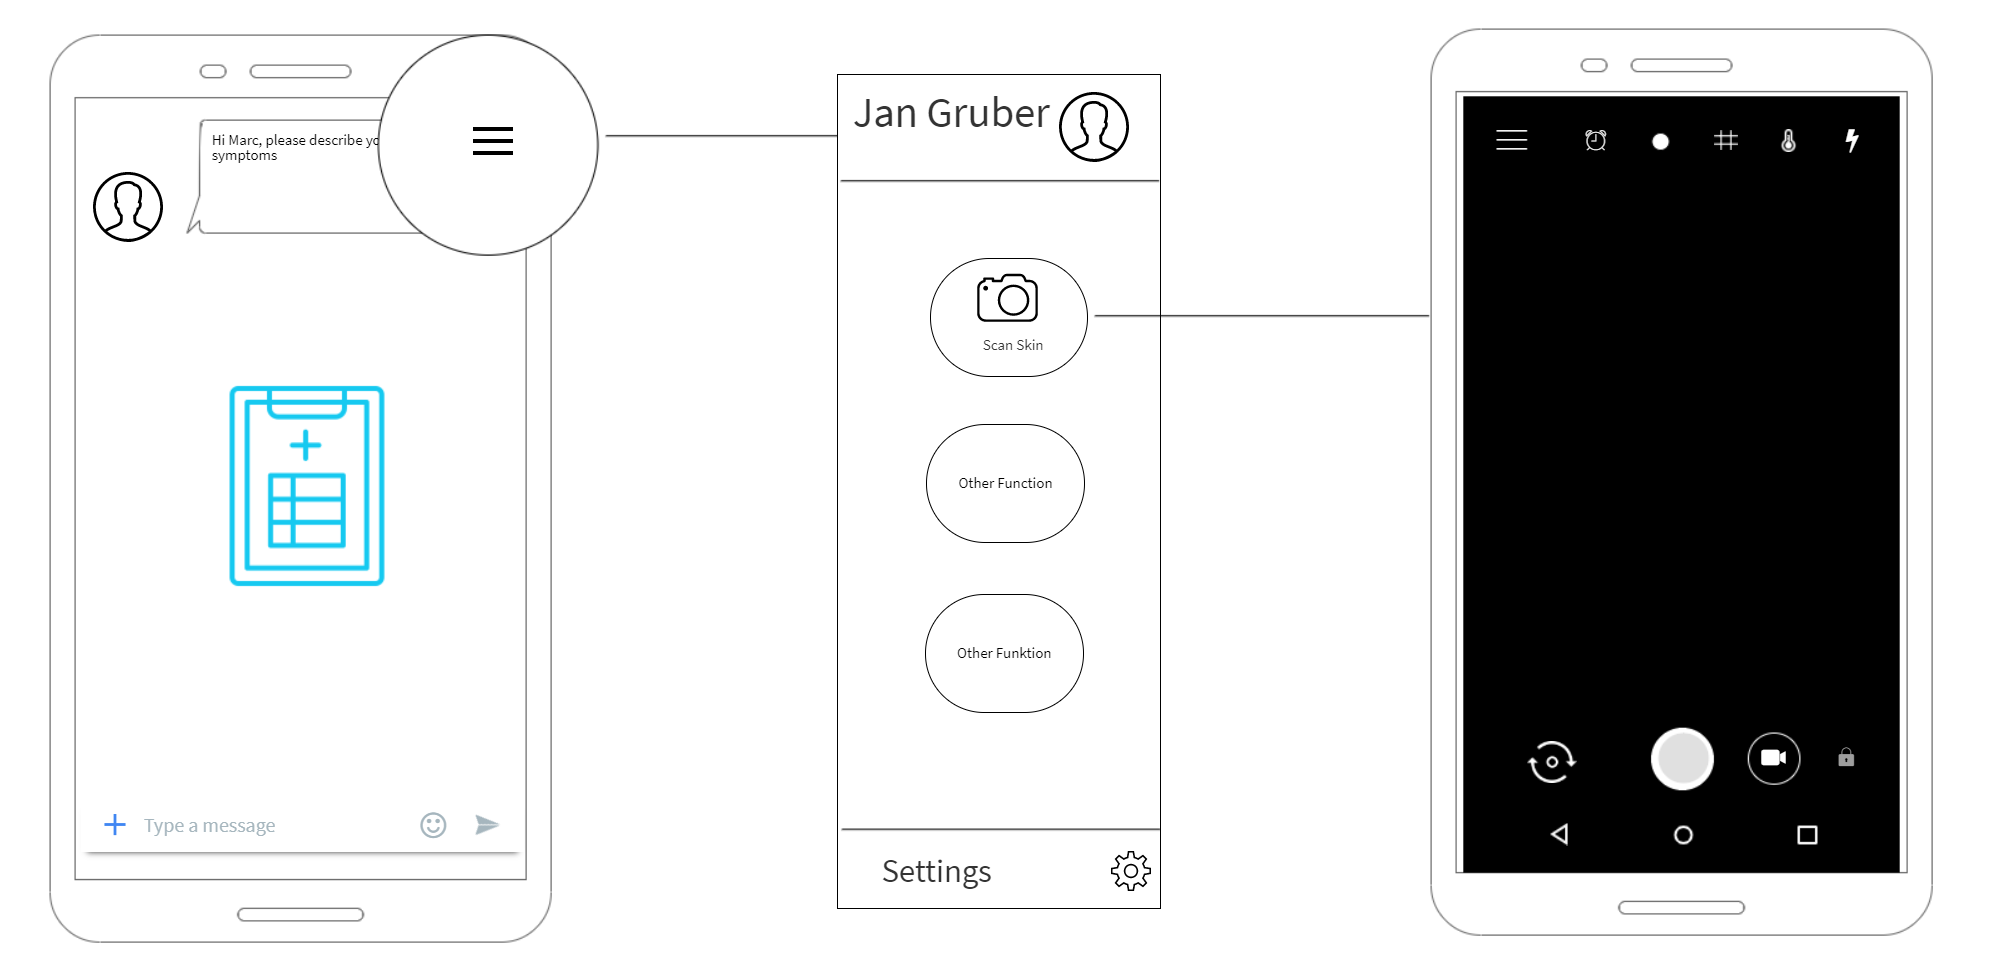
\includegraphics[scale=0.7]{SystemSpec/Usecases/Mocks/scanskin01.png}\\
        
        \item The user has already entered their somewhat skin related symptoms, so to make the diagnosis more accurate Doctor Robert suggests to try our skin scan feature and provides an option to open it right from the dialog.
        
            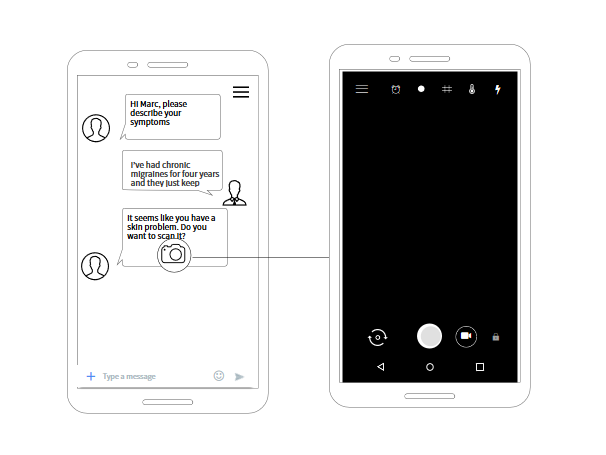
\includegraphics[scale=0.7]{SystemSpec/Usecases/Mocks/scanskin02.png}\\
            
        \end{enumerate}
    
    \subsubsection{The Standard Use}
        
        Depending on how the use case was called the happy path differs a bit, but is essentially the same:
        
       \begin{center}
            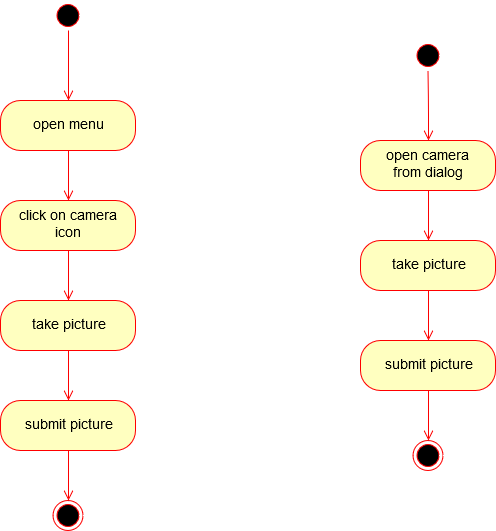
\includegraphics[scale=0.49]{SystemSpec/Usecases/Diagrams/ScanSkinActivity1.png}\\
       \end{center}{}
        
        \paragraph{open menu}
        The user clicks on the menu button and the burger menu opens.
        
        \paragraph{click on camera icon}
        The user clicks on the camera icon to open the camera.
        
        \paragraph{open camera from dialog}
        The user clicks on a button provided in the dialog from Doctor Robert, to open the camera.
        
        \paragraph{take picture}
        The user takes a picture.
        
        \paragraph{submit picture}
        The user submits the picture he took by pressing a button.
    
    \subsubsection{The Non-Standard Use}
        
        \begin{itemize}
            \item The user submits a picture of something other than skin.
            
                This is specified in \hyperlink{ScanSkinNonStandard}{GetDiagnosis}
        \end{itemize}{}
        
\pagebreak
